\documentclass{scrbook}
%\documentclass{article}
\usepackage{mdframed}
\usepackage{amsmath}
\usepackage{tikz}
\usepackage{lipsum}
\usepackage{svg}

%\usepackage[utf8]{inputenc}
%!TEX root = thesis.tex

% Set german to default language and load english as well
\usepackage[english,ngerman]{babel}

% Set UTF8 as input encoding
\usepackage[utf8]{inputenc}

% Set T1 as font encoding
\usepackage[T1]{fontenc}
% Load a slightly more modern font
\usepackage{lmodern}
% Use the symbol collection textcomp, which is needed by listings.
\usepackage{textcomp}
% Load a better font for monospace.
\usepackage{courier}
% Load package to configure header and footer
\usepackage{scrlayer-scrpage}

% Set some options regarding the document layout. See KOMA guide
\KOMAoptions{%
  paper=a4,
  fontsize=12pt,
  parskip=half,
  headings=normal,
  BCOR=1cm,
  headsepline,
  headsepline=0.5pt,
  DIV=12}

% do not align bottom of pages
\raggedbottom

% set style of captions
\setcapindent{0pt} % do not indent second line of captions
\setkomafont{caption}{\small}
\setkomafont{captionlabel}{\bfseries}
\setcapwidth[c]{0.9\textwidth}

% set the style of the bibliography
\bibliographystyle{alphadin}

% load extended tabulars used in the list of abbreviation
\usepackage{tabularx}

% load the color package and enable colored tables
%\usepackage[table]{xcolor}

% define new environment for zebra tables
\newcommand{\mainrowcolors}{\rowcolors{1}{maincolor!25}{maincolor!5}}
\newenvironment{zebratabular}{\mainrowcolors\begin{tabular}}{\end{tabular}}
\newcommand{\setrownumber}[1]{\global\rownum#1\relax}
\newcommand{\headerrow}{\rowcolor{maincolor!50}\setrownumber1}

% add main color to section headers
\addtokomafont{chapter}{\color{maincolor}}
\addtokomafont{section}{\color{maincolor}}
\addtokomafont{subsection}{\color{maincolor}}
\addtokomafont{subsubsection}{\color{maincolor}}
\addtokomafont{paragraph}{\color{maincolor}}

% do not print numbers next to each formula
\usepackage{mathtools}
\mathtoolsset{showonlyrefs}
% left align formulas
\makeatletter
\@fleqntrue\let\mathindent\@mathmargin \@mathmargin=\leftmargini
\makeatother

% Allow page breaks in align environments
\allowdisplaybreaks

% header and footer
\pagestyle{scrheadings}
\setkomafont{pagenumber}{\normalfont\sffamily\color{maincolor}}
\setkomafont{pageheadfoot}{\normalfont\sffamily}
\setkomafont{headsepline}{\color{maincolor}}

% German guillemets quotes
\usepackage[german=guillemets]{csquotes}

% load TikZ to draw diagrams
\usepackage{tikz}

% load additional libraries for TikZ
\usetikzlibrary{%
  automata,%
  positioning,%
}

% set some default options for TikZ -- in this case for automata
\tikzset{
  every state/.style={
    draw=maincolor,
    thick,
    fill=maincolor!18,
    minimum size=0pt
  }
}

% load listings package to typeset sourcecode
\usepackage{listings}

% set some options for the listings package
\lstset{%
  upquote=true,%
  showstringspaces=false,%
  captionpos=b,%
  basicstyle=\ttfamily,%
  keywordstyle=\color{keywordcolor}\slshape,%
  commentstyle=\color{commentcolor}\itshape,%
  stringstyle=\color{stringcolor}}
\renewcommand{\lstlistingname}{Quelltext}
\renewcommand{\lstlistlistingname}{Quelltextverzeichnis}

% enable german umlauts in listings
\lstset{
  literate={ö}{{\"o}}1
           {Ö}{{\"O}}1
           {ä}{{\"a}}1
           {Ä}{{\"A}}1
           {ü}{{\"u}}1
           {Ü}{{\"U}}1
           {ß}{{\ss}}1
}

% define style for pseudo code
\lstdefinestyle{pseudo}{language={},%
  basicstyle=\normalfont,%
  morecomment=[l]{//},%
  morekeywords={for,to,while,do,if,then,else},%
  mathescape=true,%
  columns=fullflexible}

% load the AMS math library to typeset formulas
\usepackage{amsmath}
\usepackage{amsthm}
\usepackage{thmtools}
\usepackage{amssymb}

% load the paralist library to use compactitem and compactenum environment
\usepackage{paralist}

% load varioref and hyperref to create nicer references using vref
\usepackage[ngerman]{varioref}
\PassOptionsToPackage{hyphens}{url} % allow line break at hyphens in URLs
\usepackage{hyperref}

% setup hyperref
\hypersetup{breaklinks=true,
            pdfborder={0 0 0},
            ngerman,
            pdfhighlight={/N},
            pdfdisplaydoctitle=true}

% Fix bugs in some package, e.g. listings and hyperref
\usepackage{scrhack}

% Allow todos
\usepackage{todonotes}

% define german names for referenced elements
% (vref automatically inserts these names in front of the references)
\labelformat{figure}{Abbildung\ #1}
\labelformat{table}{Tabelle\ #1}
\labelformat{appendix}{Anhang\ #1}
\labelformat{chapter}{Kapitel\ #1}
\labelformat{section}{Abschnitt\ #1}
\labelformat{subsection}{Unterabschnitt\ #1}
\labelformat{subsubsection}{Unterunterabschnitt\ #1}
\AtBeginDocument{\labelformat{lstlisting}{Quelltext\ #1}}

% define theorem environments
\declaretheorem[numberwithin=chapter,style=plain]{Theorem}
\labelformat{Theorem}{Theorem\ #1}

\declaretheorem[sibling=Theorem,style=plain]{Lemma}
\labelformat{Lemma}{Lemma\ #1}

\declaretheorem[sibling=Theorem,style=plain]{Korollar}
\labelformat{Korollar}{Korollar\ #1}

\declaretheorem[sibling=Theorem,style=definition]{Definition}
\labelformat{Definition}{Definition\ #1}

\declaretheorem[sibling=Theorem,style=definition]{Beispiel}
\labelformat{Beispiel}{Beispiel\ #1}

\declaretheorem[sibling=Theorem,style=definition]{Bemerkung}
\labelformat{Bemerkung}{Bemerkung\ #1}

\input{macros}

% Set title and author used in the PDF meta data
\hypersetup{
  pdftitle={Wie schreibe ich eine Masterarbeit?},
  pdfauthor={Erika Mustermann}
}

% Depending on which of the following two color schemes you import your thesis will be in color or grayscale. I recommend to generate a colored version as a PDF and a grayscale version for printing.

%!TEX root = thesis.tex

% define color of example university
%\xdefinecolor{SRH_Orange}{rgb}{0.87451, 0.28235, 0.027451}
\xdefinecolor{SRH_Orange}{RGB}{223, 72, 7}
\xdefinecolor{SRH_Blue}{RGB}{0, 105, 154}
\xdefinecolor{SRH_Warm_Grey}{RGB}{170, 163, 157}
\xdefinecolor{SRH_Sun_Yellow}{RGB}{252, 198, 30}
\xdefinecolor{SRH_Fresh_Mint}{RGB}{53, 180, 160}
\xdefinecolor{SRH_Sweet_Berry}{RGB}{202, 0, 127}
\xdefinecolor{SRH_Deep_Blue}{RGB}{2, 30, 48}
\xdefinecolor{SRH_Smokey_Black}{RGB}{87,87,86}

\colorlet{maincolor}{SRH_Orange}

\colorlet{stringcolor}{green!60!black}
\colorlet{commentcolor}{black!50}
\colorlet{keywordcolor}{maincolor!80!black}

\newcommand{\imagesuffix}{-color}
%\input{schema-gray}



\newcommand{\duedate}{15. Juli 2016}

\begin{document}
  \frontmatter
  %!TEX root = thesis.tex

\begin{titlepage}
  \thispagestyle{empty}

  \vskip1cm

  \pgfimage[height=2.5cm]{SRH-WLH}%\imagesuffix}
  
  \vskip2.5cm
  
  \LARGE
  
  \textbf{\sffamily\color{maincolor}Physik}

  \textit{Skriptum zur Vorlesung BB 258}

  \normalfont\normalsize

  \vskip5em
  
  \textbf{\sffamily\color{maincolor}Dr. Markus Walther}


  \vskip3em
  
  Version 140522


  \vfill

  
\end{titlepage}

  %\include{declaration}

  %\include{abstract}

  \cleardoublepage
  \phantomsection
  \pdfbookmark{\contentsname}{tableofcontents}
  \markboth{\contentsname}{}
  \tableofcontents

  % Remove this for the final version of the thesis!
  \cleardoublepage
  \phantomsection
  %\newcommand{\listtodoname}{Aufgabenverzeichnis}
  %\pdfbookmark{\listtodoname}{listoftodos}
  %\listoftodos[\listtodoname]

  \mainmatter
  %\include{einleitung}
  %!TEX root = thesis.tex

\chapter{Klassische Mechanik: Kraft, Bewegung und Energie}
\label{chapter-mechanik}

Die sogenannte Klassische Mechanik ist eine der Grundfesten der Physik, und Gegenstand der menschlichen Neugier seit tausenden von Jahren. Bereits die alten Griechen und Ägypter beschäftigten sich damit, denn ohne sie wäre der Bau vieler der antiken Monumentalbauten nicht möglich gewesen.

Richtig Fahrt gewann das Feld der klassischem Mechanik dann im Spätmittelalter und der Renaissance. während derer Gelehrte wie Newton, Foucault, Leibnitz und Gauss den Formalismus der Klassischen Mechanik entwickelten und auf die makroskopische Welt anwendeten. Nicht lange danach erkannte man auch, dass sehr analoge Gesetzte auch in der Mechanik der Atome und Moleküle untereinander gelten, und wie wir in \ref{chapter-materie} sehen werden dort zur Beschreibung von Phänomenen wie Wärme und Druck äußerst nützlich sind.

%\section{Kraft, was ist das?}

Wir betrachten hier den Formalismus der Mechanik nach Newton, dessen zentrales Element der Begriff der Kraft ist. 

Mit Kraft beschreibt man in der Physik das Phänomen des mechanischen Einflusses den ein Objekt auf ein anderes ausübt. Was genau diesen Einfluss bewirkt, kann durchaus unterschiedlich sein, und wird uns neben diesem Kapiel auch in \ref{chapter-materie} und \ref{chapter-qmrt} noch näher beschäftigen.

Neben den abstoßenden und anziehenden Kräften der elektrostatischen Kraft, auf die sich fast jede direkte Interaktion von Materie zurückführen lässt, gibt es auch noch die magnetische Kraft, die mit der elektrostatischen Kraft eng verwandt ist, und die Gravitationskraft. Weiterhin existieren noch die kernstarke Kraft und die kernschwache Kraft, die wir aber nicht näher betrachten werden.

\section{Newton's Gesetze}
\label{chapter-newtonslaws}

\textit{Isaac Newton (1643-1727)} hat mit seinen Gesetzen die grundlegenden Zusammenhänge zwischen Kraft (Einheit \textit{Newton (N)}) und den anderen Größen der klassischen Mechanik formuliert.

\begin{mdframed}[backgroundcolor=SRH_Warm_Grey!50,skipabove=3em,skipbelow=1em,frametitle=Newtons erstes Gesetz (Trägheitsprinzip)]
\textit{Corpus omne perseverare in statu suo quiescendi vel movendi uniformiter in directum, nisi quatenus illud a viribus impressis cogitur statum suum mutare.}

Ein Körper verharrt im Zustand der Ruhe oder der gleichförmig geradlinigen Bewegung, sofern er nicht durch einwirkende Kräfte zur Änderung seines Zustands gezwungen wird.
\end{mdframed}

Dieses Prinzip ist uns allen intuitiv eingängig, jeder weiß aus seiner Lebenserfahrung, dass Gegenstände nicht von selbst anfangen sich zu bewegen, wenn auf sie keine treibende Kraft wirkt.

\begin{mdframed}[backgroundcolor=SRH_Warm_Grey!50,skipabove=3em,skipbelow=1em,frametitle=Newtons zweites Gesetz (Aktionsprinzip)]
\textit{Mutationem motus proportionalem esse vi motrici impressae, et fieri secundum lineam rectam qua vis illa imprimitur.}

Die Änderung der Bewegung ist der Einwirkung der bewegenden Kraft proportional und geschieht nach der Richtung derjenigen geraden Linie, nach welcher jene Kraft wirkt.
\end{mdframed}

Die Bewegung (also die Geschwindigkeit $\vec{v}$, Einheit \textit{Meter pro Sekunde ($\dfrac{m}{s}$)}) eines Körpers ändert sich also proportional zur einwirkenden Kraft. Proportional bedeudet hier, dass sich bei einer Vordopplung der Kraft auch die Wirkung verdoppelt, und sich bei einer Halbierung der Kraft entsprechend die Wirkung halbiert, so dass der Zusammenhang zwischen Kraft und Änderung der Geschwindigkeit in einem Diagramm also durch eine Grade dargestellt werden kann.
\begin{eqnarray}
\dot{\vec{v}} \propto \vec{F}
\end{eqnarray}
Der Punkt über $\dot{\vec{v}}$ bedeudet \textit{Änderung von}, hier also \textit{Änderung der Geschwindigkeit}

Daraus lässt sich herleiten, dass die Änderung der Geschwindigkeit, also die Beschleunigung $\vec{a}$ (Einheit \textit{Meter pro Quadratsekunde oder Meter pro Sekunde hoch zwei ($\dfrac{m}{s^2}$))}) der Kraft dividiert durch die Masse (Einheit \textit{Kilogramm (kg)}) des beschleunigten Körpers entspricht.
\begin{eqnarray}
\dot{\vec{v}}=\vec{a}=\frac{\vec{F}}{m}
\end{eqnarray}
oder, umgestellt in die häufigfer geschriebene Form:
\begin{eqnarray}
\vec{F}=m \cdot \vec{a}
\end{eqnarray}
Quasi nebenbei haben wir damit auch den Zusammenhang zwischen Geschwindigkeit und Beschleunigung hergeleitet, nämlich dass die Beschleunigung die Änderung der Geschwindigkeit ist.
\begin{eqnarray}
\dot{\vec{v}}=\vec{a}
\end{eqnarray}

\begin{mdframed}[backgroundcolor=SRH_Warm_Grey!50,skipabove=3em,skipbelow=1em,frametitle=Newtons drittes Gesetz (Gegenwirkungsprinzip)]
\textit{Actioni contrariam semper et aequalem esse reactionem: sive corporum duorum actiones in se mutuo semper esse aequales et in partes contrarias dirigi.}

Kräfte treten immer paarweise auf. Übt ein Körper A auf einen anderen Körper B eine Kraft aus (actio), so wirkt eine gleich große, aber entgegen gerichtete Kraft von Körper B auf Körper A (reactio).
\end{mdframed}
Mathematisch formuliert lässt sich dieses Gesetz wie folgt schreiben:
\begin{eqnarray}
\vec{F}_{A\rightarrow B}=-\vec{F}_{B\rightarrow A}
\end{eqnarray}


\begin{mdframed}[backgroundcolor=SRH_Warm_Grey!50,skipabove=3em,skipbelow=1em,frametitle=Superpositionsprinzip der Kräfte]
Wirken auf einen Punkt oder starren Körper mehrere Kräfte $\vec{F}_{1},\vec{F}_{2},\vec{F}_{3},\dotsc,\vec{F}_{n}$, so addieren sich diese vektoriell zu einer resultierenden Kraft $\vec{F}$ auf.
\end{mdframed}
Zusätzlich zu seinen Gesetzten hat Newton das Superpositionsprinzip formuliert, welches sich mit der Addition, also Überlagerung von Kräften befasst, und auch zur Zerlegung verwendet werden kann. Siehe dazu auch den mathematischen Anhang in \ref{chapter-mathe}.

\section{Impuls, gleichförmige und beschleunigte Bewegung}
\label{chapter-impuls}
Entsprechend dem ersten Newtonschen Gesetz verändert sich der Bewegungszustand eines Objekts ohne äußeren Einfluss nicht. Ein Objekt, welches still steht wird auch weiterhin stehen still stehen, und Objekte die sich bewegen werden sich auch weiterhin bewegen. 

An vielen Stellen der Physik ist es aber wichtig, nicht nur den Bewegungszustand zu kennen, sondern auch den "Aufwand", der notwendig ist, um diesen Zustand zu erreichen. Diese Information ist in der Geschwindigkeit nicht enthalten.

Wenn wir uns an \ref{chapter-newtonslaws} zurück erinnern, wissen wir, dass die Kraft F die notwenig ist, um einen Geschwindigkeitszustand zu ändern dem Produkt aus Masse m und Beschleunigung a entspricht, und dass die Beschleunigung der der Änderung der Geschwindigkeit entspricht: 

\begin{eqnarray}
\vec{F}=m \cdot \vec{a}=m \cdot \dot{\vec{v}}
\end{eqnarray}

Um genau zu sein ist $\dot{\vec{v}}$ die lokale Änderung der Geschwindigkeit, also die Änderung während eines sehr kleinen Zeitraumes. 

Wenn wir statt der Änderung der Geschwindigkeit über den gesamten Einflusszeitraum aufsummieren können wir daraus eine neue Größe ableiten, den sogenannten Impuls (Einheit: \textit{Kilogramm mal Meter pro Sekunde ($\dfrac{kg \cdot m}{s}$)})

\begin{eqnarray}
\vec{p}=m \cdot \vec{v}
\end{eqnarray}

Wir summieren also quasi die Beschleunigungsanteile über die Zeit auf, so dass der Impuls p eine art Aufzeichnung oder Aufsummierung der aufgewendeten Kraft ist. Mathematisch schreibt man dies wie folgt:

\begin{eqnarray}
\vec{p}=\int \dfrac{\vec{F}}{m} dt =\dfrac{1}{m}\int \vec{F} dt 
\end{eqnarray}

Es handelt sich dabei um ein sogenanntes Integral. Vereinfacht kann man ein Integral so lesen, dass man die Größe nach dem Integralzeichen $\int$ vor dem $d$ aufsummiert, und die Größe nach dem $d$ die Grüße ist, über die man aufsummiert. $\int \dfrac{\vec{F}}{m} dt$ bedeutet also, das die Änderung der Größe $\dfrac{\vec{F}}{m}$ mit der Zeit $t$ betrachtet, und den Wert von $\dfrac{\vec{F}}{m}$ jeweils für einen kleinen Zeitabschnitt aufsummiert, so dass man in Summe die Gesamtänderung von $\dfrac{\vec{F}}{m}$ im betrachteten Zeitraum erhält.

$\vec{p}$ ist also ein Maß für den Aufwand, den man verwendet hat, um den aktuellen Bewegungszustand eines Objektes zu erhalten.

Man kann Newtons Erstes Gesetz als auch wie folgt formulieren:

\begin{mdframed}[backgroundcolor=SRH_Warm_Grey!50,skipabove=3em,skipbelow=1em,frametitle=Newtons erstes Gesetz (alternative Formulierung)]
Der Impuls eines Körpers auf den keine externen Kräfte einwirken ist konstant.
\end{mdframed}

Dies entspricht dem Zustand der gleichförmigen Bewegung.

Im Kontrast dazu spricht man von beschleunigter Bewegung, wenn eine Kraft auf den Körper einwirkt, und sich dadurch der Impuls ändert.

\begin{mdframed}[backgroundcolor=SRH_Warm_Grey!50,skipabove=3em,skipbelow=1em,frametitle=Exkurs: Wo ist der Mittelpunkt des Universums?] 
Wenn man von Stillstand und Bewegung spricht, muss man sich natürlich fragen: Relativ zu welchem Nullpunkt?
Die einfache Antwort ist: Welcher Nullpunkt auch immer am einfachsten zu verwenden ist. Es gibt keinen inherenten \textit{Nullpunkt des Universums}. Stattdessen legt man sich seinen Nullpunkt zum Problem passend fest. Das einzig Wichtige dabei ist, dass man für ein System immer den gleichen Nullpunkt verwenden muss, und dass man bei Übergang zwischen verschiedenen Systemen mit unterschiedlichen Nullpunkten alle Größen entsprechend auf den neuen Nullpunkt umrechnen muss.
\end{mdframed}

\begin{mdframed}[backgroundcolor=SRH_Warm_Grey!50,skipabove=3em,skipbelow=1em,frametitle=Exkurs: Gravitatonskraft und Gravitationsbeschleunigung] 
Gravitation erzeugt eine Kraft. Allgemein ist die Gravitation definiert als
\begin{eqnarray}
\vec{F}_{G}=\dfrac{m_1 \cdot m_2 \cdot G}{\vec{r}^2}
\end{eqnarray}
Da im Schwerefeld der Erde die Masse der Erde und der Abstand r für alle Objekte auf der Erdoberfläche annähernd gleich sind (der Radius r entspricht dem Abstand von der Erdoberfläche zum Erdmittelpunkt), kann man diese Größen mit der Gravitationskonstante G zusammenfassen. Daher ergibt sich auf der Erde eine vereinfachte Formel:
\begin{eqnarray}
\vec{F}_{G(Erde)}=m_{Objekt} \cdot g
\end{eqnarray}
mit der Gravitationsbeschleunigung $g=9.81\dfrac{m}{s^2}$. Für Überschlagsrechnungen ist oft sogar ein Wert von $10\dfrac{m}{s^2}$ ausreichend genau. Man kann daher in erster Näherung sagen, dass die Gravitationskraft auf einen Körper (knapp) dem Zehnfachen seiner Masse in kg entspricht.

Entsprechend Newtons Drittem Gesetz wirkt auf einen Körper eine der Gravitationskraft entsprechende Gegenkraft wenn er auf einer Oberfläche aufliegt, die ihn am Fallen hindert. Ist das jedoch nicht der Fall, so befindet sich der Körper im freien Fall, und in diesem Fall wirkt statt der Kraft eine Beschleunigung, die den Fall des Körpers bestimmt. Diese Beschleunigung ist die oben errechnete Gravitationsbeschleunigung $g$. Es ist in diesem Fall zu beachen, dass die Beschleunigung des Falles nicht von der Masse des Körpers abhängt. Eine Feder fällt also genaus schnell wie ein Amboss, sofern keine anderen Kräfte (wie zum Beispiel Luftwiderstand) wirken.

\end{mdframed}

\section{Energie, Arbeit und Leistung}

Man könnte an dieser Stelle annehmen, dass die kinetische Energie (Bewegungsenergie) eines Objekts dem Impuls entspricht. Dies ist jedoch nicht so. Neben dem im \ref{chapter-impuls} eingeführten und berechneten vektoriellen Impuls $\vec{p}$ hat ein Körper auch noch eine Bewegungserergie (Einheit der Energie: \textit{Joule (J)})
\begin{eqnarray}
E_{kin}=\dfrac{1}{2}m\vec{v}^2
\end{eqnarray}
Man beachte dabei, dass die Bewegungsenergie $E_{kin}$ anders als der Impuls keine vektorielle sondern eine skalare Größe ist, also keine Richtung sondern nur einen Wert besitzt.

Die Begründung warum es zwei getrennte Größen \textit{Impuls} und \textit{Bewegungsenergie} gibt, ist mit einer mathematisch relativ aufwendigen Herleitung verbunden, und soll an dieser Stelle deshalb nicht näher ausgeführt werden.

Hier kann auch der Begriff der \textit{Arbeit} $W$ eingeführt werden, die ebenfalls die Einheit \textit{Joule} hat. Arbeit ist als Änderung der Energie (hier der kinetischen Energie) definiert, und wird über das Skalarprodukt aus der Kraft $F$ und Strecke $s$ über die diese Kraft ausgeübt wird hergeleitet
\begin{eqnarray}
W = \Delta E_{kin}=\vec{F}\cdot \vec{s}
\end{eqnarray} 
Der große griechiche Buchstabe Delta, $\Delta$, bedeudet in der Physik in der Regel \textit{Gesamtänderung} oder \textit{Summe der Änderungen}.

Während die Kraft also wie grade gesehen ein Maß für die Änderung der Energie, und damit die Menge der geleisteten Arbeit \textit{im Verhältnis zur zurückgelegten Strecke} $s$ ist, brauchen wir häufig auch ein Maß für die Änderung der Energe \textit{im Verhältnis zur vergangenen Zeit} $t$. Diese Größe bezeichnet man als \textit{Leistung} $P$ (Einheit \textit{Watt (W)}). Ihre Beziehung zur Arbeit und Energie ist 
\begin{eqnarray}
W = \Delta E = P\cdot t
\end{eqnarray}
oder nach $P$ aufgelöst
\begin{eqnarray}
P = \dfrac{W}{t} = \dfrac{\Delta E}{t}
\end{eqnarray}

\section{Reibung und Luftwiderstand}

\section{Hebelgesetzte}


\section{Praktische Anwendungen im Gesundheitswesen}

\begin{mdframed}[backgroundcolor=SRH_Warm_Grey!50,skipabove=3em,skipbelow=1em,frametitle=Exkurs: Vektorzerlegung mit dem Vektorenparallelogramm] 
Anders als bei Skalaren spielt bei Vektoren die Richung eine Rolle. Oft ist es notwendig, einen Gesamtvektor in zwei Teilvektoren zu zerlegen, die entlang bestimmter Achsen verlaufen. Dies ist die Umkehrung der Vektoraddition.

Dazu zeichnet man zuerst den vorhandenen Vektor, sowie von seinem Fußpunkt aus die Richtungslinien der gewünschten Zerlegungsvektoren.  

\begin{tikzpicture}
\draw[dashed] (0,0) -- (-6,2);
\draw[dashed] (0,0) -- (2,4);
\draw[thick,->] (0,0) -- (0,3);
\end{tikzpicture}

Im zweiten Schritt Zeichnet man von der Spitze des Vektors aus Parallelen zu den beiden Richtungslinien, bis diese eine der Richtungslinien vom Fußpunkt schneiden

\begin{tikzpicture}
\draw[dashed] (0,0) -- (-6,2);
\draw[dashed] (0,0) -- (2,4);
\draw[thick,->] (0,0) -- (0,3);
\draw[dashed] (0,3) -- (2,2.33);
\draw[dashed] (0,3) -- (-1.5,0);
\end{tikzpicture}

Im letzten Schritt zeichnet man die Ergebnisvektoren ein. Diese führen vom Fußpunkt des ursprünlichen Vektors entlang der Richtungslinien bis zum Schnittpunkt mit der Parallelen von der Vektorspitze


\begin{tikzpicture}
\draw[dashed] (0,0) -- (-6,2);
\draw[dashed] (0,0) -- (2,4);
\draw[thick,->] (0,0) -- (0,3);
\draw[dashed] (0,3) -- (2,2.33);
\draw[dashed] (0,3) -- (-1.5,0);
\draw[thick,->] (0,0) -- (-1.286,0.429);
\draw[thick,->] (0,0) -- (1.286,2.571);
\end{tikzpicture}

Damit ist die Vektoraufteilung abgeschlossen, und die beiden Teilvektoren können für weitere Rechnungen verwendet werden.
\end{mdframed}

\section{Übungsaufgaben}
\emph{Lösungen siehe \ref{chapter-loesungen}}

\paragraph{Übung 1.1}

%\textbf{Übung 1.1}

Berechnen Sie, wie lange ein Fahrzeug, welches sich mit der Geschwindigkeit von $25 \frac{m}{s}$ vorwärts bewegt für eine Strecke von 100 Kilometern benötigt.

\paragraph{Übung 1.2}

Ein Fahrzeug wird aus dem Stand eine Minute lang mit einer gleichförmigen Beschleunigung $a=1.25\frac{m}{s^2}$ beschleunigt, und fährt im Anschluss mit gleichbleibender Geschwindigkeit eine Strecke von 175 Kilometern. Wie lange benötigt das Fahrzeug, um ab dem Stillstand an seinem Ziel anzukommen?

\paragraph{Übung 1.3}

Herr Müller geht mit seinem Hund Friedhelm spazieren. Leider ist Friedhelm heute nicht in der Stimmung für lange Spaziergänge, so dass Herr Müller permanent mit einer Kraft von 2N an der Leine ziehen muss, um Friedhelm zur Kooperation zu bewegen. Nach zwei Umrundungen des Häuserblocks (Seitenlänge 40m) hat Friedhelm alle notwendigen Geschäfte erledigt, und Herr Müller keine Lust mehr, so dass sich beide wieder in ihre Wohnung begeben. Wieviel Arbeit hat Herr Müller durch das Ziehen an Friedhelms Leine geleistet?

\paragraph{Übung 1.4}

Bufti Schorsch soll einen 20kg schweren Karton mit Infusionsbeuteln in den Schrank sortieren. Er möchte die Kiste dazu auf den Tisch heben, um den Inhalt leichter entnehmen zu können. Schorsch bemüht sich, den Karton rückenschonend zu heben, schafft dies aber nicht ganz. Er ist beim Heben immernoch um 10° nach vorne geneigt. Bestimmen Sie sowohl graphisch (durch Parallelogrammzerlegung) als auch rechnerisch, welche Kraft entlang Schorschs Wirbelsäule wirkt, und welche Kraft senkrecht dazu ein Biegemoment auf Schorschs Wirbelsäule ausübt.

\paragraph{Übung 1.5}

Heinz möchte auf seinem Balkon einen großen Blumentopf mit einer Palme aufstellen. Der Blumentopf ist Zylinderförmig, und hat einen Durchmesser von 50cm sowie eine Höhe von 1m. Die Palme, der Topf und die Planzerde wiegen zusammen 100kg. Im ungünstigsten Fall ist außerdem davon auszugehen, dass der Topf zusätzlich komplett mit Regenwasser voll läuft. Wasser hat eine Dichte von $1\frac{g}{cm^3}$, das heißt ein Liter Wasser wiegt 1kg. Von seinem Vermieter erfährt Heinz, dass der Balkon für eine Traglast von $5\frac{kN}{m^2}$ ausgelegt ist, die nicht überschritten werden darf. Kann Heinz seine Palme auf dem Balkon aufstellen?

\textit{Die Wandstärke des Topfes soll vernachlässigt werden\\Die Formel zur Berechnung einer Kreisfläche ist $A_{Kreis}=\pi \cdot r^2$, die zur Berechnung des Zylindervolumens $V_{Zylinder}=A_{Kreis} \cdot h=\pi \cdot r^2 \cdot h $}

\paragraph{Übung 1.6}

\paragraph{Übung 1.7}

\paragraph{Übung 1.8}

\paragraph{Übung 1.9}

\paragraph{Übung 1.10}


\paragraph{Übung 1.11}

\paragraph{Übung 1.12}

\paragraph{Übung 1.13}

\paragraph{Übung 1.14}

\paragraph{Übung 1.15}

\paragraph{Übung 1.16}

\paragraph{Übung 1.17}

\paragraph{Übung 1.18}

\paragraph{Übung 1.19}

\paragraph{Übung 1.20}
  %!TEX root = thesis.tex

\chapter{Aufbau der Materie}
\label{chapter-materie}

\begin{displayquote}
\begin{center}
\textit{Daß ich nicht mehr mit sauerm Schweiß,\\
Zu sagen brauche, was ich nicht weiß;\\
Daß ich erkenne, was die Welt\\
Im Innersten zusammenhält}
\end{center}
\begin{flushright}
\textit{Faust}, J. W. von Goethe
\end{flushright}
\end{displayquote}

\section{Woraus besteht das Universum?}

Das Universum wird in der Regel beschrieben als endlicher aber unbeschränkter Raum oder Bereich, in dem sich alle uns zugänglichen dinglichen und nicht-dinglichen Phänomene befinden.

Diese Aussage ist nach unserem Wissen richtig, aber auch verhältnismäßig inhaltsleer. Die Realität ist, dass wir nicht wissen was genau das Universum ist, worin es seinen Ursprung hat, und warum es so funktioniert wie es funktioniert. 

Wir wissen allerdings inzwischen mit relativ großer Genauigkeit, wie es funktioniert, das heißt wir können viele (aber nicht alle) Phänomene im Universum erklären und auch voraussagen. Dieses Erklären und Voraussagen ist die Domäne der Naturwissenschaften und im Speziellen der Physik. Alle anderen Naturwissenschaften können prinzipiell als Spezialisierungen der Physik auf Teilbereiche der Naturwissenschaft angesehen werden.

Aus Sicht der klassischen Physik können die uns bekannten Phenomene in zwei Gruppen aufgeteilt werden: \textit{Materie} und \textit{Kräfte}, die wir im Folgenden betrachten wollen.

\section{Materie}
\lipsum[1]
\section{Kräfte}
Wie wissen jetzt, woraus Materie besteht. Aber wie interagiert Materie miteinander? Die Phenomene, welche bei der Interaktion von Materie miteinander oder bei Veränderung der Materie auftreten, fasst man unter den Begriffen \textit{Wechselwirkungen} oder \textit{Kräfte} zusammen. Zu jeder Kraft gehört ein Überträgerteilchen, welches die Wirkung der Kraft vermittelt.

Grundsätzlich sind uns vier Wechselwirkungen bekannt.

\subsection{Die elektromagnetische Kraft}


Die Elektromagnetische Wechselwirkung wirkt zwischen elektrisch geladenen Teilchen. Ihre für uns sichtbaren Ausprägungen sind die elektrostatische Anziehung und Abstoßung, sowie die magnetische Anziehung und Abstoßung, die beide Formen der gleichen Kraft sind. Das Überträgerteilchen der elektromagnetischen Kraft ist das Photon, welches auch einzeln existieren kann.

Die elektromagnetische Kraft hat vermutlich mit den größten Einfluss auf unser Leben, sie ist dafür verantwortlich, dass feste Gegenstände nicht durcheinander hindurch fallen können, die ist eine der Treibenden Kräfte hinter chemischen Reaktionen, und ihr Überträgerteilchen, das Photon, durchdringt unser Leben in Form von Radiowellen, Licht, Röntgen- und Gammastrahlen, die alle elektromagnetische Strahlung verschiedener Frequenzen sind.

Die Reichweite der elektromagnetischen Kraft ist unbeschränkt.

Die Ausprägung als elektrostatische Kraft wird durch das Coulomb-Gesetz beschrieben:
\begin{eqnarray}
 F_C=\dfrac{1}{4\cdot\pi\cdot\epsilon_0}\cdot\dfrac{q_1\cdot q_2}{r^2}
 \end{eqnarray}
Dabei ist $\pi=3,1415...$ die Kreiszahl, $\epsilon_0=8,854188\cdot 10^{-12} \dfrac{A\cdot s}{V\cdot m}$ die elektische Feldkonstante, $q_1$ und $q_2$ die Ladungen der betrachteten Punktladungen in Coulomb (Abgekürzt C, als zusammengesezte Einheit Ampere mal Sekunde), und r der Abstand der Ladungen in Meter.

Die Kraft in der Ausprägung als Magnetismus bezeichnet man als magnetische Kraft:
\begin{eqnarray}
\vec{F}_B = q \cdot \vec{v} \times \vec{B}
\end{eqnarray}
$q$ ist dabei die Ladung in Coulomb die sich mit der Geschwindigkeit $\vec{v}$ (in Meter pro Sekunde) durch ein Magnetfeld der magnetischen Flussdichte $\vec{B}$ (Einheit Tesla, abgekürzt $T=\dfrac{kg}{A\cdot s^2}=\dfrac{V \cdot s}{m^2}$). Das $\times$ bezeichnet die mathematische Operation des Kreuzproduktes.

Zusammen bezeichnet man die Summe aus diesen beiden Kräften als Lorenzkraft

\begin{eqnarray}
\vec{F}_L=\vec{F}_C+\vec{F}_B
\end{eqnarray}


Um Verwirrung zu vermeiden ist dabei ist aber zu beachten, dass in älteren Lehrbüchern abweichend davon die magnetische Kraft $\vec{F}_B$ als Lorenzkraft $\vec{F}_L$ bezeichnet wird.  



\subsection{Die kernstarke Kraft}

Die kernstarke Kraft ist für den Zusammenhalt der Quarks, und damit der aus den Quarks gebildeten Baryonen Proton und Neutron, sowie aller anderer in der Natur normalerweise nicht frei vorkommenden aus Quarks gebildeten Teilchen (Hadronen) verantwortlich. Sie vermittelt ebenso den Zusammenhalt benachbarter Hadronen, insbesondere in Atomkernen den Zusammenhalt zwischen Protonen und Neutronen im Atomkern. 

Die Überträgerteilchen der kernstarken Kraft sind die Gluonen, von denen es 6 verschiedene Ausprägungen sowie nochmals genausoviele Antiteilchen dazu gibt.

Die Reichweite der kernstarken Kraft ist sehr klein, und liegt im Bereich des Durchmessers eines Atomkerns. Dafür ist aber ihre Energie sehr hoch. In der Regel spielt die kernstarke Kraft in unserem Alltag keine große Rolle. Die Änderung des Bindungszustandes der kernstarken Kraft in Atomkernen bei radioaktivem Zerfall, Kernspaltung und Kernfusion ist aber für die dabei frei werdenden Energiemengen verantwortlich, so dass insbesondere Kernkraftwerke sowie nukleare Waffen ohne sie nicht möglich wären.

Die Berechnung der kerstarken Kraft ist mit Rechnungen der klassischen Physik nicht möglich, dazu werden Rechenmethoden der Quantenchromodynamik und der Quantenfeldtheorie benötigt, welche den Umfang dieser Vorlesung bei weitem überschreiten, und deshalb hier nicht ausgeführt werden sollen. Bei Interesse sei auf Lehrbücher zu diesen Berechen der Physik verwiesen.

\subsection{Die kernschwache Kraft}

Die kernschwache Kraft vermittelt zwei der fünf bekannten Radioaktiven Zerfallsarten, den $\beta^+$- und den $\beta^-$-Zerfall, ausgesprochen als \textit{Beta Plus} bzw. \textit{Beta Minus}.

Ihre Überträgerteilchen sind das $W^+$-, das $W^-$-, sowie das neutrale $Z$-Boson, die alle eine sehr kurze Reichweite aber eine große Masse haben

Dabei zerfällt beim $\beta^-$-Zerfall ein down-Quark in ein up-Quark und ein $W^-$-Boson. Letzters zerfällt dann kurze Zeit später in ein Elektron und ein Elektronen-Antineutrino. Durch die Umwandlung des down- in ein up-Quark wandelt sich das Neutron, in dem sich das Quark befindet in ein Proton um.

Analog dazu zerfällt beim $\beta^+$-Zerfall ein up-Quark in ein down-Quark und ein $W^+$-Boson. Letzters zerfällt dann kurze Zeit später in ein Positron (Antielektron) und ein Elektronen-Neutrino. Durch die Umwandlung des up- in ein down-Quark wandelt sich das Proton, in dem sich das Quark befindet in ein Neutron um.

Genau wie die kernstarke Kraft kann auch die kernschwache Kraft nur mit Methoden der Quantenchromodynamik und der Quantenfeldtheorie berechnet werden. Daher gilt das oben gesagte hier ebenso.

\begin{figure}
    \centering
    \def\svgwidth{\columnwidth}
    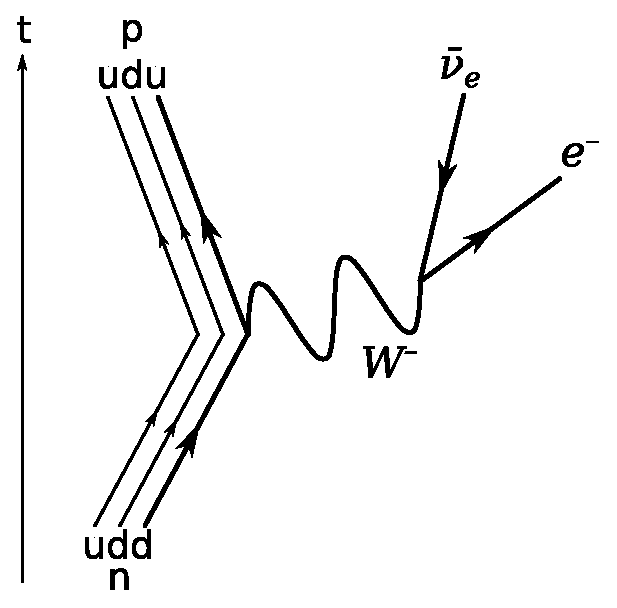
\includegraphics[scale=0.5]{Beta_Negative_Decay.eps}
    \caption{$\beta^-$-Zerfall im Feynmanndiagramm} 
\end{figure}

\subsection{Die Gravitationskraft}

Die Gravitationskraft fällt in der Gruppe der Kräft etwas aus der Reihe, da weder ihre Ursache noch das vermittelne Teilchen bisher sicher bekannt sind. Nach der Relativitätstheorie ist die Gravitation keine Kraft welche wie die anderen Kräfte durch ein Teilchen vermittelt wird, sondern eine Eigenschaft des Raumes, der durch seine Form die Masseteilchen beeinflusst. Es wird aber auch vermutet, dass es trotzdem ein Gravitationsteilchen, das Graviton, geben muss. Dieses wurde bisher aber nicht gefunden. Siehe dazu auch \ref{chapter-qmrt}.

Die Gravitation hat wie die elektromagnetische Kraft eine unbeschränkte Reichweite, ist jedoch um etliche Größenordnungen schwächer als diese oder die anderen beiden Kräfte. Der Grund für diesen extremen Unterschied ist ebenfalls nicht bekannt und Gegenstand der Forschung.

Die Gravitationskraft kann mit folgender Formel berechnet werden
\begin{eqnarray}
\vec{F}_G=\dfrac{m_1 \cdot m_2 \cdot G}{\vec{r}^2}
\end{eqnarray}

Dabei sind $m_1$ und $m_2$ die Massen der beiden Objekte die sich anziehen in Kilogramm, $G$ ist die Gravitationskonstante mit dem Wert $G=6,67430\cdot 10^{-11} \dfrac{m^3}{kg \cdot s^2}$, und $\vec{r}$ ist der Abstand der beiden Massen in Meter. Man verwendet dafür den Abstand zwischen dem Massenschwerpunkten, also den mit der lokalen Dichte gewichteten Mitten. In erster Näherung kann dafür auch die geometische Mitte der Massen verwendet werden.

\section{Statistische Thermodynamik}
\lipsum[1]
\section{Übungsaufgaben}
\lipsum[1]
  %!TEX root = thesis.tex

\chapter{Elektrotechnik: Ein spannungsgeladenes Thema}
\label{chapter-etech}


\section{Strom, Spannung}
\lipsum[1]
\section{Widerstand}
\lipsum[1]
\section{Kapazität und Induktivität}
\lipsum[1]
\section{Elektrizität in der Medizin}
\lipsum[1]
\section{Schadwirkung von Elektrizität am Körper}
\section{Übungsaufgaben}
\lipsum[1]  
  %!TEX root = thesis.tex

\chapter{Quantenfeldtheorie, das Standardmodell und die Relativitätstheorie: An vorderster Front der Forschung}
\label{chapter-qmrt}

\textit{Hinweis: Dieses Kapitel ist nicht Klausurrelevant}

\section{Quantenfeldtherie und das Standardmodell}
\lipsum[1]
\section{Relativitätstheorie}
\lipsum[1]
  
  \appendix
  %!TEX root = thesis.tex

\chapter{Anhang: Mathematische Grundlagen}
\label{chapter-mathe}


\section{Grundrechenarten}
loips
\section{Variablen: Rechnen mit Buchstaben}
lips
\section{Funktionen}
hurk
\section{Potenz, Wurzel, Logarithmus}
lops
\section{Winkel und Wellen-Trigonometre}
lups
\section{Exponentialfunktionen}
löps
\section{Vektoren}
pürp
\section{Sonstiges}
laßps
\chapter{Lösungen zu den Übungsaufgaben}
\label{chapter-loesungen}
\section{Kapitel 1}
\section{Kapitel 2}
\section{Kapitel 3}

  %!TEX root = thesis.tex

\chapter{Anhang: Weiterführende Literatur}
\label{chapter-lit}

Buch Schatz
  %\include{grundlagen}
  %%!TEX root = thesis.tex

\chapter{Konzept}
\label{chapter-konzept}

In diesem Kapitel wird die eigentliche Erkenntnis dieser Arbeit beschrieben. Der Aufbau dieses Kapitels hängt stark vom Thema der Arbeit ab. Die in dieser Vorlage vorgeschlagenen Kapitel sind auch nur als Vorschlag und auf keinen Fall als verbindlich zu verstehen.

Die folgenden Abschnitte dieses Kapitels enthalten Beispiele für die diversen Inhaltselemente einer Arbeit.\todo{Die Abschnitte dieses Kapitels sollten natürlich nicht so in die Arbeit übernommen werden.}

\todo[inline]{Notizen an einen selbst oder den Betreuer der Arbeit sind während der Arbeit sehr nützlich. Für die finale Version können diese Todo-Notes dann komplett aufgeblendet werden.}

\section{Quellen}

Quellen sind wichtig für gutes wissenschaftliches Arbeiten. Eine Quelle kann dabei zum Beispiel
\begin{compactitem}
  \item ein Beitrag in einer Zeitschrift \cite{MopOverview},
  \item ein Beitrag in einem Sammlungsband \cite{moore},
  \item ein Buch \cite{scala},
  \item ein Beitrag im Berichtsband einer Konferenz \cite{rltl},
  \item ein technischer Bericht \cite{bitkom},
  \item eine Dissertation \cite{Leucker02},
  \item eine Abschlussarbeit \cite{RltlConv},
  \item ein (noch) nicht veröffentlichter Artikel \cite{ptLTL} oder
  \item ein Artikel auf einer Website \cite{codecommit} sein.
\end{compactitem}

Dabei ist zu beachten, dass nicht veröffentlichte Artikel und insbesondere Webseiten nur in Ausnahmefällen gute Quellen sind, da diese nicht durch Fachleute begutachtet wurden.

Im Bereich der Informatik können Quellenangaben im Bib\TeX-Format direkt der dblp\footnote{\url{https://dblp.org}} entnommen werden. Dabei am besten oben rechts im Auswahl-Menü \emph{condensed} und nicht \emph{standard} oder \emph{with crossref} auswählen, damit nur die relevanten Daten enthalten sind.

Andere Dienste wie zum Beispiel Google Scholar haben zwar oft ebenfalls einen Bib\TeX-Export, dieser wird aber meistens automatisch aus anderen Metadaten generiert und ist entsprechend mit Vorsicht zu genießen. Die Daten in der dblp werden manuell von Menschen gepflegt und aktualisiert und sind entsprechend sehr oft tatsächlich korrekt.

\section{Tabellen}

In \vref{tbl-prozessoren} sehen wir ein Beispiel für eine Tabelle.

\begin{table}
  \centering
  \begin{zebratabular}{llr}
    \headerrow Jahr & Prozessor & MHz \\
    1975 & 6502 (C64) & 1 \\
    1985 & 80386 & 16 \\
    2005 & Pentium 4 & 2\,800 \\
    2030 & Phoenix 3 & 7\,320\,000 \\
    \hiderowcolors
    2050 & \ldots \\
    2070 & \ldots
  \end{zebratabular}
  \caption[Rechengeschwindigkeit von Computern]{Rechengeschwindigkeit von Computern. Inhaltlich vollkommen egal, ist dies doch ein sehr schönes Beispiel für eine Tabelle.}
  \label{tbl-prozessoren}
\end{table}

\section{Abbildungen und Diagramme}

In \vref{fig-flower} sehen wir ein Beispiel für eine Abbildung, die aus einer externen Grafik geladen wurde. In \vref{fig-buechi} sehen wir ein Beispiel für eine Abbildung, die in \LaTeX\ generiert wurde.

\begin{figure}
  \centering
  \pgfimage[width=.5\textwidth]{flower}
  \caption[Kurzfassung der Beschreibung für das Abbildungsverzeichnis]{Lange Version der Beschreibung, die direkt unter der Abbildung gesetzt wird. Es ist wichtig, für jede Abbildung eine umfangreiche Beschreibung anzugeben, da der Leser beim ersten Durchblättern der Arbeit vor allem an den Abbildungen hängen bleibt.}
  \label{fig-flower}
\end{figure}

\begin{figure}
  \centering
  \begin{tikzpicture}[
      node distance=15ex,
      auto,
      on grid,
      shorten >=1pt
    ]
    \node [state, initial] (q0) {$q_0$};
    \node [state, accepting, right=of q0] (q1) {$q_1$};
    \path[->]
      (q0) edge node {$a$} (q1);
  \end{tikzpicture}
  \caption[Graph des Büchi-Automaten $\hat A$.]{Graph des Büchi-Automaten $\hat A$. Der Zustand $q_1$ hat dabei keine ausgehende Kante. Der Zustand ist trotzdem akzeptierend, da beide enthaltenen Zustände von $\acute A$ akzeptierend sind. Die naive Anwendung des Leerheitstests auf alternierenden Büchi-Automaten liefert in diesem Fall also zu viele akzeptierende Zustände.}
  \label{fig-buechi}
\end{figure}

\section{Quelltext}

Quelltext sollte in Abschlussarbeiten nur äußerst sparsam eingesetzt werden. Wichtig ist insbesondere, dass Quelltextauszüge sorgsam ausgewählt und gut erklärt werden.

\begin{lstlisting}[language=Java,gobble=2]
  public class Main {
    // Hello Word in Java
    public static void main(String[] args) {
      System.out.println("Hello World");
    }
  }
\end{lstlisting}

\subsection{Quelltext mit automatischer Nummerierung}

Manchmal möchte man Quelltext eher als Abbildung und nicht als Fließtext behandeln. In diesem Fall soll der Quelltext eine Bildunterschrift und eine automatische Nummerierung erhalten. Die automatische Nummerierung kann dann natürlich auch in Referenzen verwendet werden: In \vref{lst:java} haben wir Java-Quelltext.

\begin{lstlisting}[language=Java,gobble=2,caption={Ich bin die Bildunterschrift des Quelltextes},label=lst:java]
  public class AnotherClass {
    private int number = 0;
    public void add() {
      this.number++;
    }
  }
\end{lstlisting}

Wenn man Quelltext mit Bildunterschrift setzt, muss man darauf achten, dass der Quelltext nach wie vor nicht als Fließumgebung behandelt wird. Entsprechend kann es passieren, dass der Quelltext über zwei Seiten hinweg gesetzt wird. Während das normalerweise nicht stört, kann dieser Umstand in Zusammenhang mit einer Bildunterschrift den Leser irritieren.

\section{Pseudocode}

Um Algorithmen zu erklären ist Pseudocode viel besser geeignet als Quelltext. Im Pseudocode kann man alles unwichtige weglassen und sich auf die mathematische Modellierung des Algorithmus konzentrieren. So kann die Struktur des Verfahrens unabhängig von Implementierungsdetails des jeweiligen Frameworks erklärt werden.

\begin{lstlisting}[style=pseudo,gobble=2]
  // Schleife von 1 bis 5
    for $i \gets 1$ to $5$ do
      while $S[i] \neq S[S[i]]$ do
        $S[i] \gets S[S[i]]$
\end{lstlisting}

\section{Formeln mit \pdfepsilon}

Das $\epsilon$ in der Überschrift dieses Abschnitts ist ein Beispiel für ein mathematisches Symbol, dass in den PDF-Lesezeichen als reiner Text gesetzt wird. Siehe \texttt{macros.tex}. In dieser Datei wird auch $n \in \N$ definiert.

Wir wissen aus der Analysis, dass
\begin{align}
  f(x) &= x^2 + px + q
\end{align}
Nullstellen bei
\begin{align}
  x_1 &= -\frac p2 + \sqrt{\frac{p^2}4 - q} \text{ und}\\
  x_2 &= -\frac p2 - \sqrt{\frac{p^2}4 - q}
\end{align}
hat.

\section{Theoreme}

\begin{Definition}[Definition]
  Eine \emph{Definition} ist die Bestimmung eines Begriffs oder eines mathematischen Zusammenhangs.
\end{Definition}

\begin{Lemma}[Unwichtiger Hilfssatz]
  \label{lem:hilfssatz}
  Der Satz \ldots
\end{Lemma}

\begin{proof}
  \ldots und sein Beweis.
\end{proof}

\begin{Theorem}[Wichtiger Satz]
  \label{thm:wichtig}
  Ein wichtiger Satz.
\end{Theorem}

\begin{proof}
  Der Beweis folgt unter Verwendung der Erkenntnisse aus \vref{lem:hilfssatz}.
\end{proof}

\begin{Korollar}[Ein Geschenk]
  Eine unmittelbare Folgerung.
\end{Korollar}

\begin{proof}
  Die Folgerung folgt unmittelbar aus \vref{thm:wichtig}.
\end{proof}

\begin{Beispiel}
  Ein Beispiel.
\end{Beispiel}

\begin{Bemerkung}
  Beispiele und Bemerkungen werden nicht in das Verzeichnis der Theoreme und Definitionen aufgenommen.
\end{Bemerkung}

\section{Anführungszeichen}

Malte sagt: \enquote{Fritz hat gesagt: \enquote{Man kann wörtliche Rede verschachteln.}}

Anführungszeichen werden nur für wörtliche Rede oder direkt übernommene kurze Zitate verwendet. Für die Hervorhebung von neu eingeführten Fachbegriffen eignet sich \emph{kursiver Satz} besser.

  %\include{evaluation}
  %\include{fazit}

  

  %\include{appendix}

  \backmatter

  \cleardoublepage
  %\phantomsection
  %\pdfbookmark{\listfigurename}{listoffigures}
  %\listoffigures

  %\cleardoublepage
  %\phantomsection
  %\pdfbookmark{\listtablename}{listoftables}
  %\listoftables

  %\cleardoublepage
  %\phantomsection
  %\renewcommand{\listtheoremname}{Definitions- und Theoremverzeichnis}
  %\pdfbookmark{\listtheoremname}{listoftheorems}
  %\listoftheorems[ignoreall,show={Lemma,Theorem,Korollar,Definition}]

  %\cleardoublepage
  %\phantomsection
  %\pdfbookmark{\lstlistlistingname}{listoflistings}
  %\lstlistoflistings

  %\include{abkuerzungen}

  %\cleardoublepage
  %\phantomsection
  %\pdfbookmark{\bibname}{bibliography}
  %\bibliography{literature}
\end{document}
